Im Rahmen des Wahlpflichtfaches ''Objective-C/Cocoa'' musste eine Anwendung für das iPhone bzw. iPad erstellt werden. Dabei sollte auch wenn möglich die Besonderheiten von IOS wie z.B. der Lagesensor, GPS und Touch-Funktionen mitverwendet werden.\\
\\
Wir haben uns Entschlossen eine neue Art Fehlersuchspiel zu entwickeln. Dieses lehnt sich an die bekannten Fehlersuchspiele in Zeitschriften an, bei denen zwei auf den ersten Blick identische Bilder nebeneinander zu sehen sind, wobei eines davon mehrere Veränderungen enthält, welche zu finden sind (siehe Abbildung \ref{fehlersuchspiel}). In ''iPad Spot The Difference'' liegt jedoch die Besonderheit, dass das Fehlerbild ein Foto aus der Realität ist und um die Fehler zu finden, dass auf dem Display dargestellten Foto auch mit der realen Umgebung verglichen werden muss.

\begin{figure}[H]
  \centering
  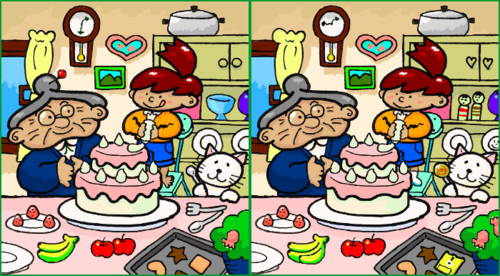
\includegraphics[width=0.6\textwidth]{bilder/Spot_the_difference.png}
  \caption{Typisches Fehlersuchbild in Zeitschriften}
  \label{fehlersuchspiel}
\end{figure}

Der Spieler erhält zu Beginn eine Weltkarte angezeigt, auf der alle Punkte markiert sind, für diese ein Fehlerbild existiert. Befindet sich der Spieler in der örtlichen Nähe einer solchen Markierung kann er das Fehlerbild mit der realen Umgebung vergleichen und die Fehler durch einen Klick auf das Bild aufdecken.\\
\\
Das Spiel wurde speziell für das iPad entwickelt, da eine möglichst großes Display nötig ist, um auch die Fehler zu erkennen.